\chapter{Implementation}\label{ch:implementation}
We implemented \trussFabName{} as a plug-in for the 3D modeling software \textit{SketchUp}. It is primarily written in Ruby and JavaScript.\unsure{Do we assume TrussFormer is a new product, which uses similar functionality as TrussFab, or do we say it is an improvement?}

\section{Architecture}
The software can be divided into four components. The most user-facing one is the designer. The other components handle the physics simulation of the created structures, minimization logic for the created hubs and hinges and the 3D print export.\\
\\
\subsection{Designer}
All components are stored in a graph structure. The building parts are \textit{Edges}, \textit{Nodes} and \textit{Triangles}. They all inherit \textit{GraphObject}. The purpose of these objects is providing user-facing functionalities and storing lower-level components. An overview of the graph structure can be seen in \ref{fig:graph}.\\
The \textit{Graph} is implemented as a Singleton \improvement{explain what a Singleton is} that stores and provides access to all GraphObjects, creates new ones and provides convenience functions for user interactions, such as finding the node closest to the mouse cursor. As this class is a singleton, every module of the software has access to the objects.\\
Each of these objects has access to its underlying logic-bearing component, called \textit{SketchupObject}.\improvement{Clarify. Either explain what that means (Hubs, Links, Surfaces) or at least have a forward reference} The access to this functionality is, however, not implemented in this superclass, but in each subclass, having the specific name as an accessor. This design decision was made to improve code readability, and decrease coding errors caused by accessing the wrong SketchupObject.\improvement{Show before and after code snippet}\\
\begin{figure}
    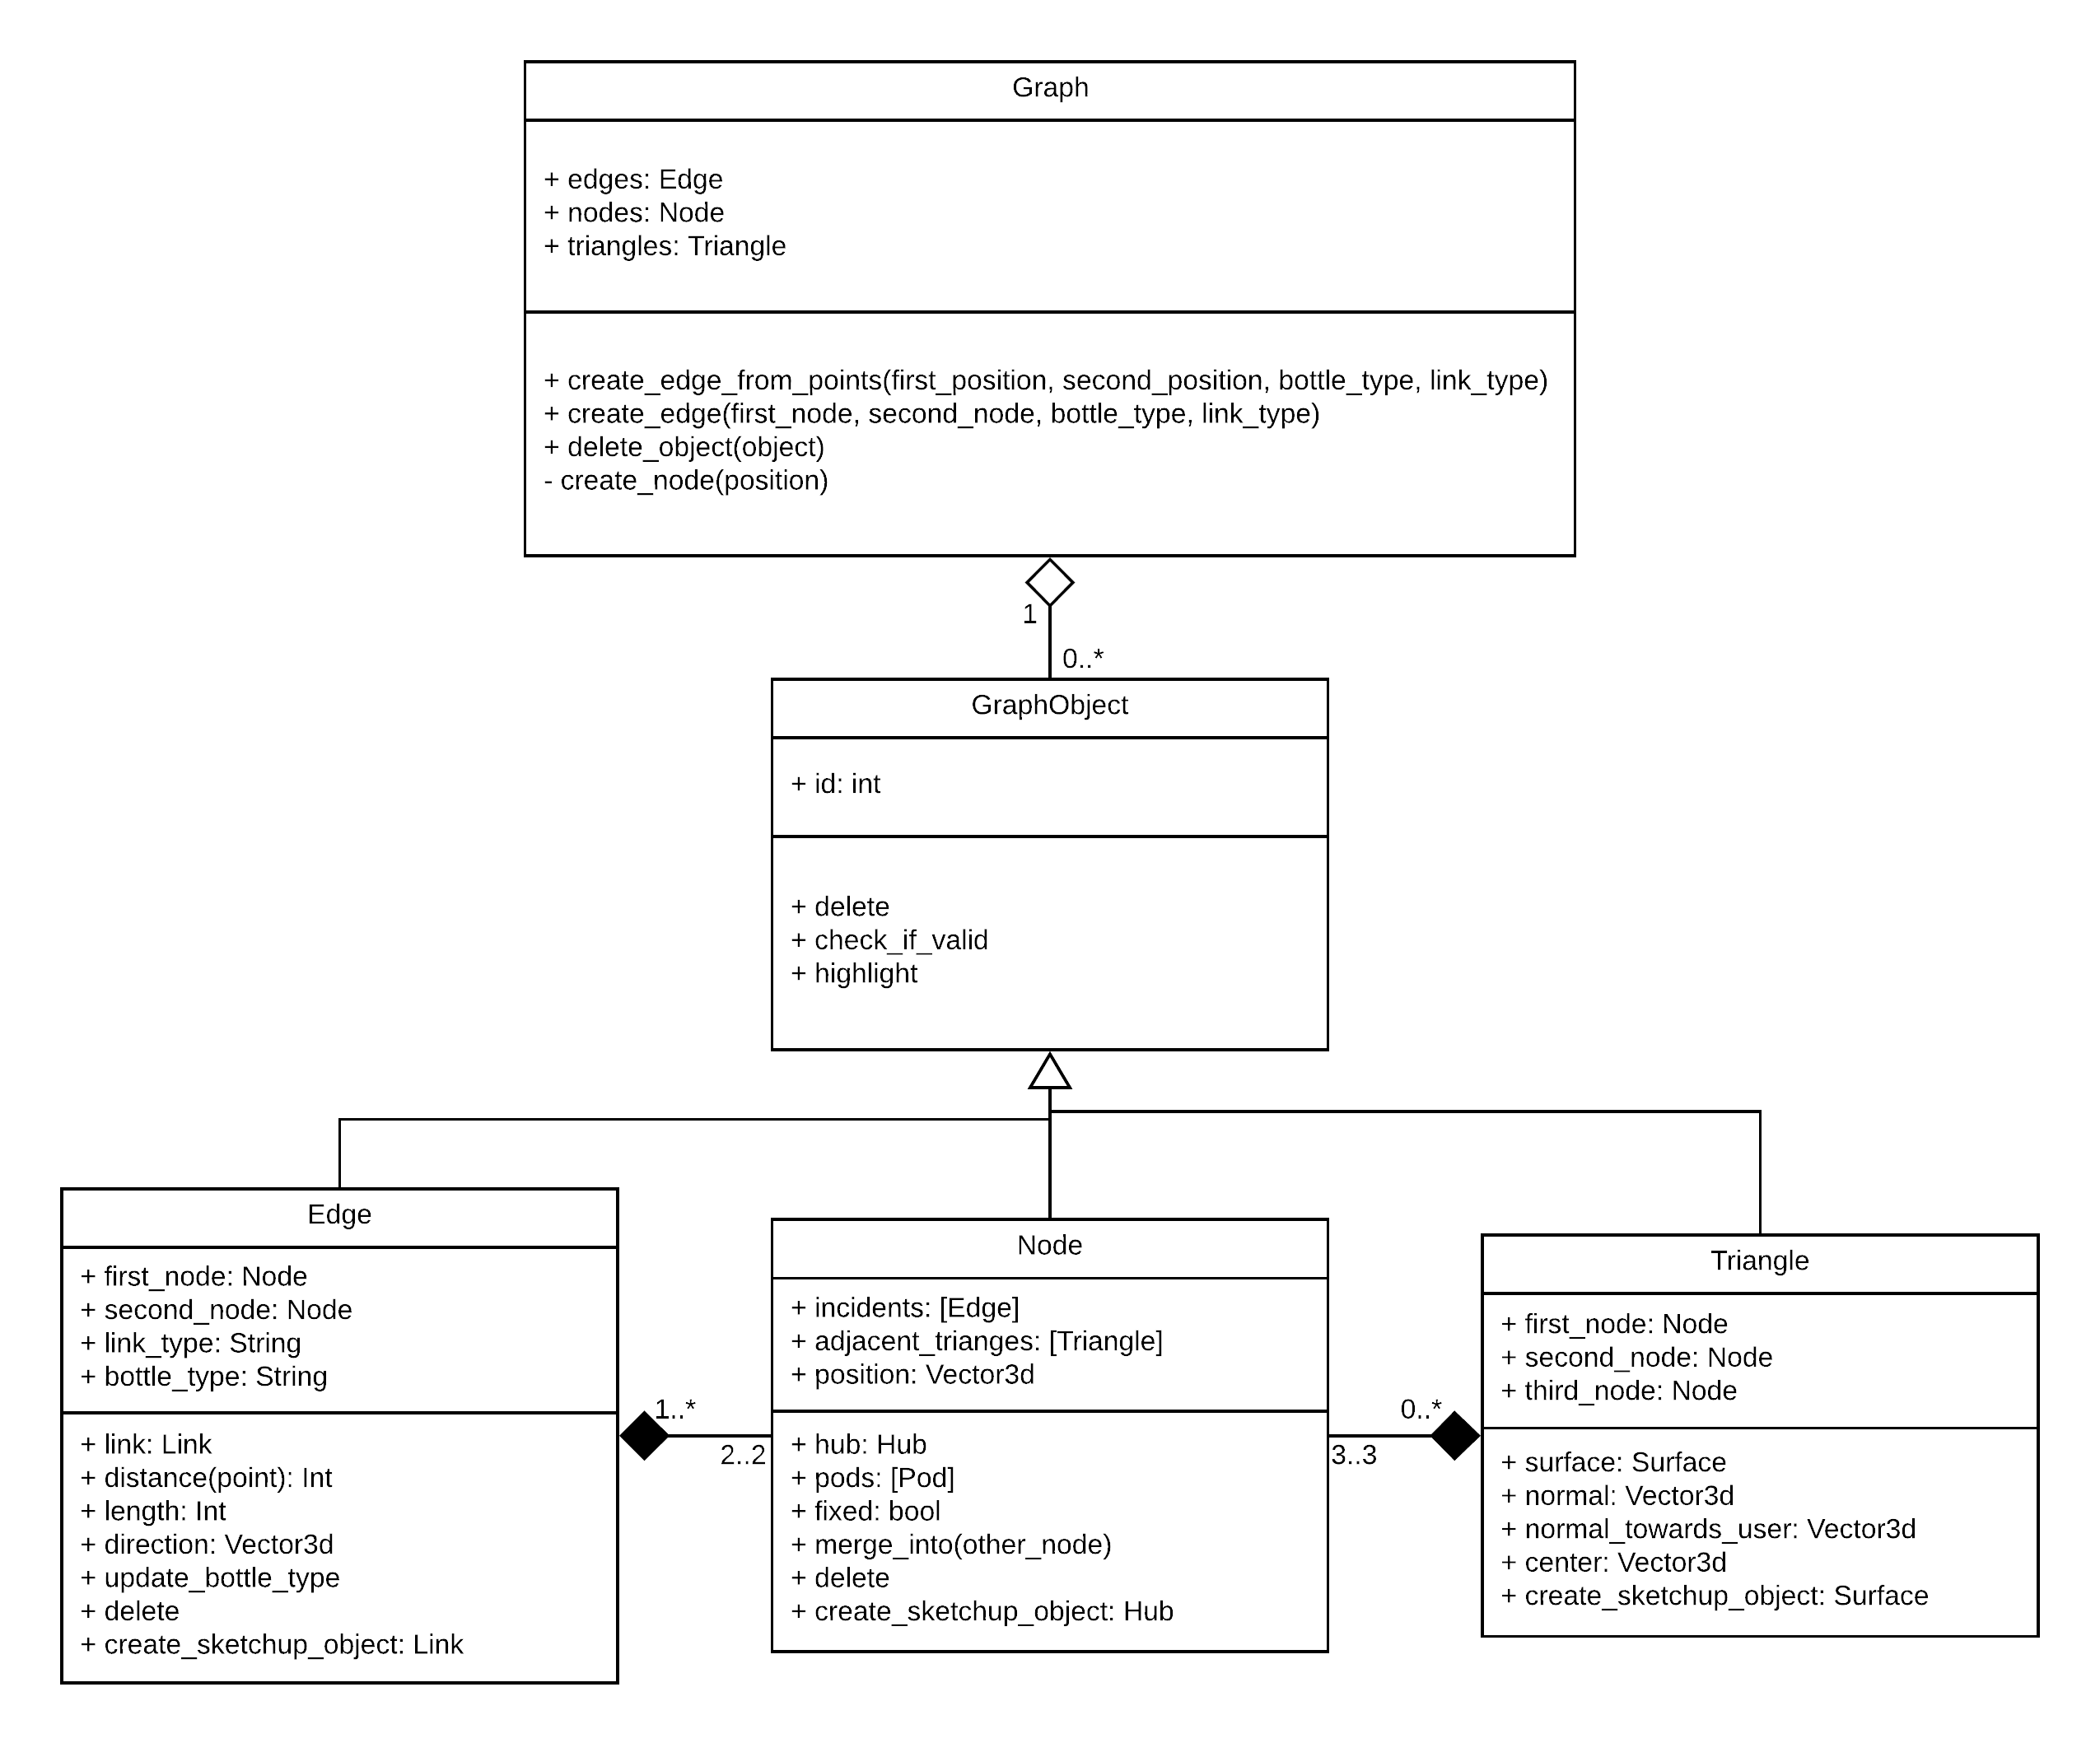
\includegraphics[width=\textwidth]{Implementation/TrussFab_Graph.png}
    \centering
    \caption{Class Diagram showing the high-level Graph Structure of the TrussFab Designer}
    \label{fig:graph}
\end{figure}
The responsibility of the GraphObject class is primarily unifying the way the appearance in SketchUp of the underlying object can be changed as much as possible. This includes highlighting a specific object if the mouse hovers over it, resetting the object to its default state and creating and deleting it. More complex methods need to be implemented in the respective subclass.\\
\textit{Nodes} are the connecting components of the structure. \textit{Edges}, as well as \textit{Triangles} are created based on Nodes. Apart from storing adjacent Edges and Triangles, a Node can specify their positions in the SketchUp world. The Nodes' adjacent objects constantly check if their position has changed and update their SketchUp representation accordingly. If the structure is deformed in such a way that a Node will be at the same position as another one, the Node object can automatically merge into the other Node. The Node will iterate over all its adjacent Edges and tell each one, apart from the Edges that run from the other Node to the Edge the Node is hinging around (i.e. the Edge that is opposite the Node), to exchange itself with the Node it wants to merge into. These Edges are removed from its own adjacent Edges and added to the collection of the new Node. The same happens for all adjacent Triangles. As a last step, the Node deletes itself and all remaining adjacent Edges and Triangles (which will be the Edges and Triangles that got merged). The object will then be adapted according to the new positions using the \textit{Relaxation algorithm}, described in section \ref{relaxation}.\\
\clearpage
\begin{lstlisting}[language=Ruby, caption=Merging of two Nodes]
  def merge_into(other_node)
    merged_incidents = []
    @incidents.each do |edge|
      edge_opposite_node = edge.opposite(self)
      next if other_node.edge_to?(edge_opposite_node)
      edge.exchange_node(self, other_node)
      other_node.add_incident(edge)
      merged_incidents << edge
    end
    @incidents -= merged_incidents

    merged_adjacent_triangles = []
    @adjacent_triangles.each do |triangle|
      new_triangle = triangle.nodes - [self] + [other_node]
      next unless Graph.instance.find_triangle(new_triangle).nil?
      triangle.exchange_node(self, other_node)
      other_node.add_adjacent_triangle(triangle)
      merged_adjacent_triangles << triangle
    end
    @adjacent_triangles -= merged_adjacent_triangles

    delete
  end
\end{lstlisting}\label{merging_code}
Another component that is tightly coupled to Nodes are \textit{Pods}. A Pod acts as a stand for the object and tells TrussFab that this Node should not change its position.\todo{add image}\\
The \textit{Edges} are the most visual components of TrussFab. They are visualized by bottles of different lengths, if they are static links, or as two cylinders forming an actuator, if they can have variable lengths. The Edges handle creating the correct model and changing it if the user decides to place a different kind of Edge. Edges play a big role in the simulation.
The last high-level component in TrussFab is the \textit{Triangle}. A Triangle is primarily used as a convenient access to multiple Nodes or Edges. Most tools that work on Nodes, such as the \textit{Add Weight Tool}, can also be applied to Triangles, adding weight to all three connected Nodes. The Triangle also provides functions for telling the \textit{MouseInput} in where a certain face is directed.\improvement{IMPROVE!}
\\- tight coupling to SketchUp (uses SketchUp Elements, SketchUp rendering engine, ...)
\subsection{Physics Simulation}
- Based on \textit{MSPhysics} by Anton Synytsia
- Ruby wrapper around C++ physics engine \textit{Newton Dynamics}
- Implemented as a \textit{SketchUp Animation}
- implements \textit{nextFrame} method
- this method is called every time SketchUp has finished rendering a frame
- this method does:
\begin{enumerate}
    \item tell Sketchup to render new frame (SketchUp will render the positions calculated in the previous world update: make use of calculate new update while sketchup already renders new positions)
    \item call \textit{update\_world}, which does, world\_iterations times:
    \begin{itemize}
        \item update forces, i.e. call apply predetermined forces (e.g. weights on hubs, calculations of PID controller)
        \item call \textit{world.advance}: Tell MSPhysics, that a new world update is available and let it calculate new forces after positional updates
        \item record tensions on links, for visualization later. This has to be recorded, because for each render step, a number of world updates are done. We don't want to miss crucial force updates
        \item visualize forces: send color information to SketchUp, indicating the strength of the tension on links
    \end{itemize}
    \item update entity positions: tell SketchUp where components have to be rendered next time
    \item send data to ui: send sensor data to ui charts, if needed
\end{enumerate}
\subsection{Minimization Logic}
- elongates and shortens edges so that maximum movement is possible with minimum material use\\
- uses iterative relaxation algorithm, will be explained in \ref{relaxation}

\subsection{Export}

\section{TrussFab Designer}
The TrussFab Designer provides static sketching functionalities. It can create and display different predefined models, has knowledge about the connections of different components and can modify the resulting objects structure.

\subsection{User Interface}

\subsection{Structure Creation}
Terminology:\\
\begin{enumerate}
    \item Edge:
    \begin{enumerate}
        \item Connects two nodes
        \item Can be:
        \begin{enumerate}
            \item Bottle Link
            \item Actuator
            \item PID link
        \end{enumerate}
    \end{enumerate}
\end{enumerate}

\subsection{Modifying the Structure}

\subsection{Relaxation Algorithm}\label{relaxation}

\subsection{OpenSCAD Export}\label{sec:openscad_impl}

\section{TrussFormer Physics Engine}

\subsection{Simulation}
- only hubs are simulated to improve performance

\subsection{Automatic Actuator Placement (if it works soon-ish)}

\section{Force Control}

\subsection{PID}
